\documentclass[pdflatex,sn-mathphys-num]{sn-jnl}
\usepackage{graphicx}
\usepackage{multirow}
\usepackage{amsmath,amssymb,amsfonts}
\usepackage{amsthm}
\usepackage{mathrsfs}
\usepackage[title]{appendix}
\usepackage{xcolor}
\usepackage{textcomp}
\usepackage{manyfoot}
\usepackage{booktabs}
\usepackage{algorithm}
\usepackage{algorithmicx}
\usepackage{algpseudocode}
\usepackage{listings}
\usepackage{tabularx}
\usepackage{array}

\raggedbottom

\begin{document}

\title[Wildfire Risk Prediction in Kazakhstan]{An Explainable Multisource Machine Learning Framework for Spatiotemporal Wildfire Risk Prediction and Mapping in Kazakhstan}

\author{\fnm{Samat} \sur{Zharylkap}}

\author{\fnm{Nurbek} \sur{Bolarbek}}

\affil{\orgdiv{School of Data Science and Artificial Intelligence}, \orgname{Astana IT University}, \orgaddress{\city{Astana}, \country{Kazakhstan}}}

\maketitle

\section{Introduction}\label{sec:introduction}

A wildfire is an uncontrolled fire that burns vegetation, such as grass, shrubs, or trees. Its development depends on fuel, moisture, weather, and an ignition source. Wildfire occurrence prediction estimates whether a new event is likely within a specific area and time. It differs from detection, which identifies a fire that has already started, and spread prediction, which estimates how an existing fire may move \cite{xu2025deep}. 

Our motivation comes from the large wildfire that began in June 2023 in the Semei Ormany reserve in Kazakhstan's Abay Region. The disaster caused the deaths of 14 forestry workers and required emergency action \cite{sentinel2023abayfire}. It raised an important question for our research: could reliable daily risk information help authorities prepare before dangerous conditions develop into a major emergency? A prediction model cannot guarantee that a fire will not start, and this study cannot establish that a model would have prevented the 2023 disaster. However, trustworthy forecasts could support closer monitoring, preparedness, and response planning. This possibility motivates our focus on locally relevant predictions rather than only general hazard maps.

The environmental context also supports this idea. Some studies explain that climate, vegetation, land use, and human activity jointly shape fire patterns.\cite{jones2022fireclimate}. In Central Asia also found frequent combined drought and heatwave events in north-central Kazakhstan and linked compound conditions with vegetation losses \cite{ding2026vegetation}. These studies does not predict fires, but it supports considering weather, vegetation, and moisture together.

Related studies provide several useful starting points. \cite{kondylatos2022danger} used Long Short-Term Memory (LSTM) and Convolutional LSTM (ConvLSTM) networks to predict next-day wildfire danger in the Eastern Mediterranean using weather, vegetation, and human-related data. \cite{jadouli2024morocco} developed a multisource dataset for Morocco and evaluated machine-learning models, including XGBoost and LightGBM, alongside feedforward neural networks for localized wildfire prediction. In Kazakhstan, \cite{babu2025sfri,chepashev2025maxent} provide national fire-risk and hazard-mapping frameworks. These studies show the value of regional data and machine learning. However, they do not test the combined reliability of daily probabilities, explanations, and transfer across Kazakhstan's regions and future seasons.

The purpose of this study is to fill these gaps and develop and evaluate an explainable multisource machine-learning framework for next-day vegetation-fire occurrence prediction and mapping in Kazakhstan. Unlike image detection or broad hazard mapping alone, this work will study whether daily probabilities remain useful across time and geography. Its target is the first satellite detection of a new event, which is a practical indicator rather than an exact record of ignition. 

The research will address the following questions:
\begin{enumerate}
\item Does combining weather, vegetation, terrain, land-cover, and human-related variables improve next-day prediction compared with seasonal fire frequency and a weather-only model?
\item How well do the models perform on future years and geographically separate regions of Kazakhstan?
\item Are the predicted probabilities well calibrated, and which factors explain the model outputs across different regions and land-cover groups?
\end{enumerate}

The proposed approach uses Kazakhstan data from 2015--2024, combining observations from NASA's Fire Information for Resource Management System (FIRMS) and the Visible Infrared Imaging Radiometer Suite (VIIRS) with weather, vegetation, terrain, land-cover, and dated human-related information\cite{nasaFirmsFaq}. The study will compare Logistic Regression, Random Forest, XGBoost, and CatBoost against seasonal fire frequency and a weather-only logistic models under the same data and validation conditions. It will also examine whether vegetation, human-related information, and recent weather history add value beyond simpler reference models. These comparisons will connect model performance with the information used, rather than assuming that a more complex method is always better. Evaluation combines average precision (AP), F1, Brier skill, calibration checks, and uncertainty estimates.

The value of this study is practical as well as methodological. The Abay Region disaster gives the research a clear national motivation, but the proposed framework will consider Kazakhstan as a whole. Reliable daily information could help identify locations that need closer monitoring and support the planning of prevention activities. Explanations could help users check whether predictions reflect reasonable environmental patterns. 

The proposed contribution is substantial because data quality, fair testing, probability reliability, and explanations are considered together. The value of the work will depend on honest comparisons and reproducible evidence, including negative results if the proposed models do not improve on simpler approaches. The contributions of this work can be summarized as follows:
\begin{itemize}
\item To prepare a Kazakhstan-specific spatial and temporal dataset that combines fire detections with environmental and human-related information, using only inputs available before the target day.
\item To compare four machine-learning models with seasonal and weather-only baselines, and test the added value of selected predictor groups.
\item To evaluate future-year and geographic transfer using temporal and spatial separation, appropriate rare-event measures, and statistical uncertainty estimates.
\item To assess and improve probability calibration and use SHAP to explain predictive associations without treating them as causal effects.
\item To produce daily probability maps and document data preparation, model settings, limitations, and evaluation steps to support reproducibility.
\end{itemize}

This work is structured as follows: Section~\ref{sec:literature_review} presents related work on wildfire prediction, multisource data, explainability, and regional research. Section~\ref{sec:methods} describes the methods and materials, including research design, datasets, preparation, models, and evaluation. Section~\ref{sec:results} presents the experimental results and discusses them in relation to the research questions, previous studies, and limitations. Finally, Section~\ref{sec:conclusion} summarizes the findings and directions for future work.

\section{Literature Review}\label{sec:literature_review}

Wildfire occurrence reflects the interaction of combustible vegetation, moisture availability, weather, ignition sources, and landscape structure. Prediction consequently requires more than identifying hot or dry conditions: it must account for where fuel is available, how its condition changes, and where ignition is likely. Remote sensing and machine learning (ML) offer complementary capabilities, providing repeated environmental observations and modeling nonlinear relationships among heterogeneous predictors \cite{xu2025deep,ejaz2025pipeline}. Nevertheless, the reliability of a predictive map depends on its target, observational labels, and validation design rather than on algorithmic complexity alone.

Occurrence forecasting, susceptibility mapping, detection, and spread prediction represent distinct tasks. Susceptibility describes spatial predisposition to fire; forecasting introduces a defined future time interval; detection identifies an existing fire; and spread modeling estimates subsequent propagation. Satellite-based reviews and spread-modeling surveys illustrate why their outputs and performance measures are not directly interchangeable \cite{ghali2023satellite,andrianarivony2024spread}. Moreover, occurrence probability represents only one component of risk. Exposure and vulnerability determine whether a hazardous event threatens people, infrastructure, or ecosystems \cite{dossi2026infrastructure}. This distinction is essential when interpreting probability maps as decision-support products.

\subsection{Multisource Observations and Fire Drivers}

Satellite observations provide both fire labels and environmental predictors. Thermal anomalies indicate active burning, whereas vegetation indices, land cover, surface temperature, and moisture products characterize fuel condition. Their integration with precipitation, humidity, temperature, wind, and terrain allows models to represent interactions between environmental dryness and spatial susceptibility \cite{xu2025deep,mambile2024systematic}. However, a thermal detection is an observation of combustion, not necessarily an ignition record. Persistent burning, agricultural fires, industrial heat, and missed observations complicate label construction. Models trained on these labels must therefore distinguish the intended vegetation-fire target from the satellite observation process \cite{ejaz2025pipeline}.

Localized dataset construction addresses another source of uncertainty. \cite{jadouli2024morocco} integrate vegetation, soil moisture, meteorological, and population-related observations for next-day prediction in Morocco, demonstrating that regional data preparation is itself a substantial contribution. \cite{ahajjam2025alaska} link spatiotemporal clustering with ensemble prediction in Alaska, highlighting the relevance of event organization when repeated detections describe the same fire. These approaches suggest that dataset quality requires coherent spatial and temporal units, not simply a larger collection of hotspot records.

Weather and fuel indicators represent related but non-identical processes. Temperature, humidity, precipitation, and drought affect drying; vegetation indices describe vegetation condition; soil moisture represents antecedent water availability; and wind influences potential propagation. \cite{mambile2024systematic} identify CNNs and LSTMs as frequently used architectures and emphasize meteorological and satellite-derived predictors, while \cite{xu2025deep} distinguish time-series, segmentation, and spatiotemporal formulations. Both reviews support heterogeneous data integration, but architecture classifications do not establish that one model is universally preferable across these tasks.

Human-access variables complement environmental predictors because favorable burning conditions do not necessarily produce ignition. Road proximity, settlements, population density, and land use may describe human pressure, although they can also correlate with reporting and observation intensity. \cite{iban2024shap} examine contributing factors through SHAP-based susceptibility mapping, while \cite{bouzeraa2025wsm} integrate GIS and ML in a regional predictive framework. Their relevance lies in connecting spatial predictions with identifiable drivers. The broader reviews identify anthropogenic information and reproducibility as areas requiring further development \cite{mambile2024systematic,galvanlara2026systematic}.

\subsection{Predictive Models and Spatial Outputs}

Tree ensembles are attractive for tabular environmental data because they accommodate nonlinear interactions without requiring image-based inputs. Deep networks instead offer representations suited to imagery and sequential observations. \cite{ejaz2025pipeline} place both within a pipeline spanning acquisition, preprocessing, feature engineering, evaluation, mapping, and deployment. \cite{galvanlara2026systematic} similarly examine algorithmic configurations, data practices, and reproducibility, indicating that fair comparison must control task definitions and experimental conditions. \cite{biswas2025geoai} directly compare deep and ML ensembles for California susceptibility prediction, providing a relevant comparative setting rather than justification for assuming that deeper architectures are automatically superior.

\cite{gupta2024geospatial} apply U-Net, DeepLabV3, and pyramid scene parsing networks to geospatial wildfire-risk modeling using imagery and environmental layers. Their contribution is a spatial modeling proof of concept; its applicability depends on the quality and meaning of the reference risk layers. \cite{ouazri2026catboost} combine CatBoost and Transformer components with meteorological, fire-danger, and satellite observations and report 92.5\% accuracy and ROC-AUC of 0.972 in Northern Morocco. These results support hybrid prediction and explanation, but do not establish equivalent operational performance under a different regional distribution or natural event prevalence.

\cite{choi2026burnedarea} address a different question: where an existing ignition is likely to burn. Their U-Net spatial allocation and boosted area-regression components produce a burn-probability field using terrain, fuel, and meteorology. Per-fire precision--recall AUC reaches 0.429 against 0.321 for the strongest baseline, while aggregate calibration error is 0.025. The explicitly evaluated probability field is a strength, but high-probability overconfidence and limited representation of suppression and spotting restrict fine-scale interpretation. Its contribution informs probability-map evaluation without substituting for pre-ignition occurrence forecasting.

Hybrid physical--ML systems seek greater behavioral structure. \cite{benhamza2025hybrid} connect neural ignition prediction with Cellular Automata propagation, joining predicted ignition locations to a spatial simulation. \cite{jadouli2026physics} embed entropy-inspired environmental representations within a neural network and examine fire-triangle feature organization. These studies connect prediction with domain knowledge, although physical inspiration alone does not establish mechanistic validity or geographic transferability. \cite{saleem2025neuralxgb} combine neural feature extraction and XGBoost for multiclass disaster classification. That architecture offers a related methodological idea, but its multi-disaster target cannot be treated as direct evidence of wildfire-occurrence forecasting skill.

\subsection{Generalization, Calibration, and Explanation}

Rare-event imbalance makes accuracy insufficient: a model may classify most non-fire observations correctly while missing consequential fires. \cite{camacho2026resampling} investigate resampling with ML for rare, high-impact wildfire prediction, demonstrating the importance of sampling design. However, large-fire prediction and general occurrence prediction concern different targets. Precision, recall, precision--recall AUC, and evaluation at realistic prevalence are therefore needed alongside discrimination measures \cite{ejaz2025pipeline,mambile2024systematic}. Calibration adds a separate requirement: probability magnitude should correspond to observed frequency, not merely rank locations correctly \cite{choi2026burnedarea}.

Spatial autocorrelation and temporal dependence also complicate validation. Neighboring locations or repeated detections can make random splits insufficient evidence of transfer to new regions or future seasons. Reviews identify geographic bias, heterogeneous resolutions, distribution shifts, and inconsistent benchmarking as persistent obstacles \cite{xu2025deep,ejaz2025pipeline,galvanlara2026systematic}. Comparison should consequently distinguish within-region interpolation from temporal forecasting and spatial transfer, while preventing information from future observations or preprocessing stages from entering training.

Explainability makes these checks more interpretable, but does not replace them. SHAP-based regional studies identify associations between predictors and model outputs, not necessarily causal ignition mechanisms \cite{iban2024shap,ouazri2026catboost}. \cite{apostolakis2025interpretation} connect daily occurrence prediction with probability-based susceptibility levels and representative sampling for local explanations. This strengthens the link between model output and usable maps. Nevertheless, stable explanations across held-out regions and seasons are more informative than feature rankings derived only from the training distribution.

\subsection{Kazakhstan Context and Research Implications}

Kazakhstan already has relevant national-scale wildfire research. \cite{babu2025sfri} integrate a Random Forest static hazard component with dynamic fire-weather, NDVI, and fuel-moisture information in a spatiotemporal fire-risk index. \cite{chepashev2025maxent} develop a machine-learning and remote-sensing fire-hazard map. These contributions establish regional precedents; therefore, novelty cannot be claimed simply from applying ML in Kazakhstan. A more defensible direction is to examine the integration of time-specific occurrence probabilities, anthropogenic information, regional transfer, calibration, and explanations within a common evaluation framework.

\cite{nurtas2026kazakhstan} review satellite-based DL for environmental-disaster detection with a Kazakhstan focus, situating wildfire analysis within wider optical and radar applications. Its broader hazard scope supports regional data and transfer considerations but does not independently demonstrate wildfire forecasting performance. Likewise, \cite{wilkjakubowski2026hazard} synthesize digital monitoring across fires, floods, earthquakes, and air pollution, connecting prediction with sensors and monitoring technologies. Operational usefulness requires timely observations and reliable workflows as well as retrospective predictive skill.

Finally, probability maps should remain distinct from comprehensive impact assessments. \cite{dossi2026infrastructure} identify infrastructure-sector gaps and the need to connect hazard, exposure, vulnerability, and interdependencies. \cite{berchtold2025tipping} introduce management tipping points to explain why extreme events can overwhelm conventional measures and require layered strategies. These perspectives support spatial decision assistance while cautioning against interpreting occurrence probability as a complete measure of expected loss.

Taken together, existing research supports localized multisource modeling but leaves important questions about label quality, human influences, transferability, probability reliability, and interpretation. For Kazakhstan, the central research need is not an unnecessarily complex architecture, but an explainable spatiotemporal framework whose probabilities remain credible across locations and seasons. Such a focus connects environmental prediction with interpretable mapping without presupposing the methodology or claiming outcomes before empirical evaluation.

\section{Methods and Materials}\label{sec:methods}

\subsection{Research Design}

The proposed study will use a quantitative, retrospective modeling design with controlled computational experiments. The objective is to estimate the probability of a newly detected vegetation-fire event within a Kazakhstan grid cell during the following day. This design is appropriate because satellite archives and environmental records permit repeated evaluation across regions and seasons without conducting hazardous ignition experiments. The framework will adapt multisource dataset construction and comparative learning from regional wildfire studies, while strengthening temporal separation and probability evaluation \cite{jadouli2024morocco,ouazri2026catboost,babu2025sfri}. All procedures below describe a planned study; no model performance or completed experiment is assumed.

\paragraph{Prediction target and scope.}
The initial analysis will cover 2015--2024 on a national equal-area grid with 5\,km cells. This resolution balances national computational requirements against the approximately 9\,km native resolution of ERA5-Land; interpolation will not be interpreted as additional meteorological detail \cite{munozsabater2021era5land}. A 1\,km regional sensitivity experiment may subsequently examine aggregation effects. Daily intervals will use UTC consistently throughout the historical record. All months will be retained initially, with seasonal performance reported separately rather than assuming that winter detections are impossible. For eligible cell $i$ and target day $t$, the model will estimate
\begin{equation}
\hat p_{i,t}=P(y_{i,t}=1\mid\mathbf{x}_{i,\leq t-1}),
\end{equation}
where $y_{i,t}$ denotes the first satellite detection of an event and the predictors contain only information timestamped before the target day. Satellite first detection is a proxy, not proof of the true ignition time. Agricultural or prescribed burning cannot always be distinguished from uncontrolled wildfire; cropland results will therefore be reported separately. The output represents occurrence hazard, not expected damage or a complete exposure--vulnerability assessment.

\paragraph{Event construction and sampling.}
VIIRS detections will first be deduplicated and linked into events through spatial and temporal proximity, following the event-oriented principle used in \cite{ahajjam2025alaska}. Initial linkage settings will be 2\,km and 48 hours, with 1--5\,km and 24--72-hour sensitivity tests. These values are proposed settings rather than thresholds established for Kazakhstan. Only the earliest detection of each connected event will define its positive cell-day. At the daily prediction cutoff, cells with a detection during the preceding 48 hours will be temporarily excluded from the new-event risk set; this exclusion uses past observations only. Event grouping may use later detections to identify repeated observations for labeling, but those later observations will never enter predictors.

All eligible positives will be retained. To reduce storage and training costs, negative cell-days will be sampled within month and broad land-cover strata using documented inclusion probabilities $q_h$. Approximately ten negatives per positive will be targeted, with a minimum allocation to strata containing no observed fires. Inverse-inclusion weights $1/q_h$ will represent the original risk set. Sensitivity analyses will compare this weighting with training-only class weighting. Validation and test data will remain unbalanced; if complete evaluation is computationally infeasible, probability-sampled evaluation will use corresponding weights. Absence of a detection will be described as an observed negative, not independently verified absence of fire.

\paragraph{Models and experimental controls.}
Four classifiers will be compared: L2-regularized logistic regression, Random Forest, XGBoost, and CatBoost. Logistic regression provides an interpretable reference, while tree ensembles accommodate nonlinear interactions and heterogeneous predictors, consistent with regional comparison studies \cite{iban2024shap,ouazri2026catboost}. Additional references will include a smoothed land-cover--calendar-month fire-frequency predictor and a weather-only logistic model. All methods will receive identical splits and feature information. Experiments will remove anthropogenic variables, lagged weather features, and vegetation information separately to quantify their incremental value. Resampling will be considered only inside training folds, informed by \cite{camacho2026resampling}; synthetic samples will not be allowed in evaluation sets. A neural--boosting architecture is not required merely because it has performed well on a different multiclass disaster task \cite{saleem2025neuralxgb}.

\paragraph{Validation, tuning, and calibration.}
Data from 2015--2021 will constitute model-development data. Hyperparameters will be selected through rolling-origin validation, for example training through 2018 and validating on 2019, then extending training for successive validation years through 2021. Fifty Optuna trials per ensemble will explore tree depth, minimum leaf size, learning rate, regularization, and estimator count, selecting weighted average precision. Early stopping will use development-fold validation only. After model selection, each classifier will be fitted on all development years. The year 2022 will be reserved for sigmoid probability calibration and decision-threshold selection; 2023--2024 will remain untouched until final evaluation.

A separate five-fold spatial-block experiment within the development period will assess geographic transfer. Initial 100\,km blocks will be grouped into geographically separated folds, with a 25\,km exclusion buffer around held-out blocks. Block-size sensitivity will test 50 and 150\,km partitions. Preprocessing and tuning will be repeated within each fold. This design separates temporal forecasting from spatial transfer and extends the geographic holdout principle examined in physics-embedded wildfire modeling \cite{jadouli2026physics}. Probability calibration will use representative or inverse-probability-weighted 2022 data rather than a balanced sample.

\paragraph{Explanation and mapping.}
TreeSHAP will explain the selected tree ensemble using global mean absolute contributions, dependence plots, and local examples from high-scoring and misclassified cells \cite{iban2024shap}. Explanations will refer explicitly to the uncalibrated model score or log-odds, not automatically to calibrated probabilities. Correlated predictor groups will also be examined together. Contributions will be compared across land-cover groups and held-out regions; they will be interpreted as predictive associations rather than causal effects. Daily calibrated probabilities will be exported directly to GeoTIFF and inspected in QGIS without interpolating point predictions. Following the probability-based mapping motivation of \cite{apostolakis2025interpretation}, class boundaries will be selected on calibration data and fixed before testing, with continuous probabilities and observed class frequencies retained.

\subsection{Data Sources}

\paragraph{Fire observations and quality control.}
NASA FIRMS archived, standard-processed Suomi-NPP VIIRS 375\,m active-fire observations will provide the primary labels. Using one primary sensor reduces changing-sensor coverage effects. Nominal- and high-confidence detections will be retained; low-confidence records will be excluded. VIIRS confidence categories will not be treated as MODIS percentage values \cite{nasaFirmsFaq}. Coordinates, dates, confidence, and available source-type fields will be checked. Persistent industrial hotspots will be screened against mapped non-vegetated locations, with the mask specified using development-period evidence only. MODIS observations and burned-area products will provide corroboration rather than indiscriminately adding detections to the target. Official incident records, if obtainable with permission, will serve as supplementary verification. They are not assumed to be available, and sample counts will be reported only after extraction.

\paragraph{Environmental predictors.}
ERA5-Land hourly fields will supply temperature, dewpoint, wind components, precipitation, and surface-layer soil moisture \cite{munozsabater2021era5land}. Daily temperature extrema, mean wind speed, relative humidity derived from temperature and dewpoint, and precipitation totals will be calculated before the target day. Accumulated precipitation will be converted according to the product's accumulation conventions. Seven- and fourteen-day antecedent precipitation and temperature summaries will represent drying history. Any optional fire-weather index will be computed exclusively from earlier observations or introduced as a clearly documented archived product, not as target-day realized weather.

MODIS MOD13A2 Version 6.1 will provide 1\,km, 16-day NDVI and EVI with quality masks \cite{nasaMod13a2}. A composite will enter predictors only after its full observation interval has ended, using an additional conservative publication lag recorded in the data manifest. Annual MCD12Q1 land cover will be used as fractions of forest, grassland, shrubland, cropland, and other classes; the preceding year's map will be preferred to avoid contemporaneous retrospective labeling. SRTM terrain will supply elevation, slope, and aspect. Population density, settlement proximity, and road proximity will be obtained from dated WorldPop products and historical OpenStreetMap snapshots where available. Present-day road data will not be silently substituted for historical conditions; unavailable historical layers will be omitted from the primary experiment and clearly identified in sensitivity analyses.

\paragraph{Preparation, availability, and resources.}
All layers will be clipped to an authoritative Kazakhstan boundary and aligned to a documented equal-area projection. Continuous layers will be area-averaged or interpolated appropriately; categorical layers will be summarized as area fractions. Slope will be derived at native terrain resolution before aggregation. Vegetation gaps will use the latest valid historical value for at most 32 days, after which missingness will be preserved. Numeric imputation, scaling for logistic regression, categorical encoding, and feature screening will be fitted on training partitions only. Strongly correlated features will be assessed with grouped ablations rather than automatically removing physically informative fire drivers. The multisource preparation strategy follows regional dataset and geospatial modeling approaches \cite{jadouli2024morocco,gupta2024geospatial}.

The core inputs are publicly accessible under provider-specific terms; public access does not imply unrestricted redistribution. No personal-level or self-collected data are required. Python, pandas, xarray, GeoPandas, rasterio, scikit-learn, XGBoost, CatBoost, Optuna, SHAP, and QGIS will support processing and analysis. Google Earth Engine may assist raster extraction, subject to account access and quotas. A multicore workstation with approximately 32\,GB RAM and SSD storage is a proposed starting configuration, not a claim about available hardware. Partitioned Parquet files and chunked raster processing will control memory use; larger runs may use approved cloud resources. Actual hardware, package versions, random seeds, source identifiers, exclusions, and split manifests will accompany the final reproducibility record.

\subsection{Evaluation Metrics}

Evaluation will distinguish discrimination, classification decisions, probability reliability, and spatial usefulness. At threshold $\tau$, weighted or complete-risk-set confusion counts will give
\begin{equation}
\mathrm{Precision}=\frac{TP}{TP+FP},\quad
\mathrm{Recall}=\frac{TP}{TP+FN},\quad
F_1=\frac{2TP}{2TP+FP+FN}.
\end{equation}
Accuracy will be reported for comparability, but not used for selection. False-positive rate, $FP/(FP+TN)$, and false-discovery proportion, $FP/(TP+FP)$, will be reported separately because they answer different warning-reliability questions. Threshold selection will maximize weighted calibration-year $F_1$, accompanied by recall--precision tradeoffs; no threshold will be optimized on test outcomes.

Average precision (AP) will be the primary threshold-independent measure:
\begin{equation}
\mathrm{AP}=\sum_k(R_k-R_{k-1})P_k,
\end{equation}
where $P_k$ and $R_k$ are precision and recall at successive score thresholds. AP will be distinguished from trapezoidally integrated PR-AUC. Event prevalence will accompany every result because it defines the no-skill precision reference. ROC-AUC will supplement AP but cannot alone establish useful rare-fire warnings. This evaluation emphasizes the rare-class information highlighted by probabilistic wildfire studies \cite{choi2026burnedarea}.

Probability quality will be measured with the weighted Brier score and skill relative to the seasonal reference:
\begin{equation}
\mathrm{BS}=\frac{\sum_n w_n(\hat p_n-y_n)^2}{\sum_n w_n},\qquad
\mathrm{BSS}=1-\frac{\mathrm{BS}}{\mathrm{BS}_{\mathrm{reference}}}.
\end{equation}
Positive BSS indicates improvement over the reference. Reliability diagrams and ten-bin expected calibration error will compare mean probabilities with observed weighted event frequencies. Bin counts and uncertainty will be shown because an apparently small aggregate calibration error can conceal unreliable high-score bins \cite{choi2026burnedarea,jadouli2026physics}.

Map usefulness will be assessed by the proportion of detected event starts captured within the highest-scoring 5\%, 10\%, and 20\% of eligible cell-days, alongside the area and false-alert burden. Scores will be stratified by year, month, region, and land-cover group. Paired 95\% confidence intervals for model differences will use 1,000 space--time block-bootstrap resamples, retaining predictions from every model on identical resampled units. Training time, inference time, and peak memory will also be recorded. Success will mean improved AP over both references, positive Brier skill, acceptable calibration, and geographically consistent gains--not achieving an arbitrary published accuracy on a different dataset. Negative or unstable improvements will be reported explicitly.


% ---------------------------------------------------------------------------
% Results and Discussion, Conclusion: drafted with AI assistance (Claude) as a
% research-organizing and review aid from the study's own experiment outputs.
% Check your instructor's policy on AI use before submitting any of this text.
% ---------------------------------------------------------------------------
\section{Results and Discussion}\label{sec:results}

All values reported below come from the study's own retrospective experiment for 2015--2024; no simulated, imaginary, or adapted results are used. Unless stated otherwise, metrics refer to the untouched test years 2023--2024, and intervals are paired 95\% space--time block-bootstrap intervals (1,000 resamples of 100\,km $\times$ 30-day blocks).

\subsection{Dataset, implementation, and model selection}\label{sec:res_data}

The national grid contains 110,129 cells of 5\,km. Table~\ref{tab:dataset} lists the new-event starts and prevalence by year. Fire activity declined over the decade: prevalence fell from $3.2$--$5.4\times10^{-4}$ in the development years to $1.5\times10^{-4}$ in 2024, so every model was tested on rarer events than it was trained on.

\begin{table}[htbp]
\caption{New-event starts and prevalence by year and role}\label{tab:dataset}
\centering\footnotesize
\setlength{\tabcolsep}{3pt}
\begin{tabularx}{\textwidth}{@{}l l >{\centering\arraybackslash}X >{\centering\arraybackslash}X >{\centering\arraybackslash}X@{}}
\toprule
Year & Role & New-event starts & Eligible cell-days ($\times10^{6}$) & Prevalence ($\times10^{-4}$) \\
\midrule
2015 & Development & 15,326 & 40.1 & 3.82 \\
2016 & Development & 13,050 & 40.2 & 3.24 \\
2017 & Development & 21,819 & 40.1 & 5.44 \\
2018 & Development & 14,844 & 40.1 & 3.70 \\
2019 & Development & 18,773 & 40.1 & 4.68 \\
2020 & Development & 16,679 & 40.2 & 4.15 \\
2021 & Development & 12,951 & 40.1 & 3.23 \\
2022 & Calibration & 10,134 & 40.1 & 2.52 \\
2023 & Test & 9,563 & 39.8 & 2.40 \\
2024 & Test & 6,187 & 40.3 & 1.54 \\
\bottomrule
\end{tabularx}
\par\smallskip\raggedright\scriptsize All positives are retained; eligible cell-days are inverse-inclusion weighted totals of the sampled negatives and positives.
\end{table}

The experiment followed the planned design with documented changes (Table~\ref{tab:implementation}). The most consequential concerns weather timing. ERA5 is published about five days late, so daily weather entered as day $t-7$ and the antecedent windows ended on $t-7$ \cite{hersbach2020era5,openmeteoOpenData}. This keeps every input available before the target day, but it weakens the meteorological signal.

\begin{table}[htbp]
\caption{Planned design (Section~\ref{sec:methods}) and its implementation}\label{tab:implementation}
\centering\footnotesize
\setlength{\tabcolsep}{3pt}
\begin{tabularx}{\textwidth}{@{}l X X@{}}
\toprule
Component & Planned & Implemented \\
\midrule
Weather & ERA5-Land (9\,km), observations before $t$ & ERA5 (0.25$^{\circ}$) from the Open-Meteo archive \cite{hersbach2020era5,openmeteoOpenData}; day $t-7$ and 7/14-day windows ending $t-7$ \\
Vegetation & MOD13A2 NDVI/EVI, 16-day & NOAA CDR NDVI (0.05$^{\circ}$), weekly, used $\geq$12 days after observation \cite{noaaCdrNdvi} \\
Human pressure & Dated WorldPop, OSM roads & WorldPop 2010 \cite{worldpop2010}; distance to Natural Earth settlements \cite{naturalEarthPlaces}; no roads \\
Tuning & 50 Optuna trials per ensemble & 5 trials (budget amended before test access) \\
Spatial blocks & 50, 100, 150\,km; re-tuned per fold & 100\,km with 25\,km buffer; hyperparameters fixed \\
Ablation & Human, lagged weather, vegetation & Seven predictor groups and a weather-only model, refitted post hoc \\
\bottomrule
\end{tabularx}
\end{table}

Rolling-origin validation selected XGBoost, with mean AP of 0.0191 over 2019--2021. CatBoost followed at 0.0110 and Random Forest at 0.0090. Logistic regression (0.0021), the seasonal reference (0.0018), and the weather-only model (0.0009) trailed. The ranking was identical in each validation year and on the test years, so model choice did not depend on a single season.

\subsection{Predictive performance against the reference models}\label{sec:res_performance}

The test prevalence of $1.96\times10^{-4}$ defines the no-skill AP. XGBoost reached an AP of 0.0204 (95\% CI 0.0166--0.0311), about 104 times the no-skill level (Table~\ref{tab:performance}, Fig.~\ref{fig:pr}). It exceeded the seasonal reference by 0.0161--0.0306 AP and the weather-only model by 0.0162--0.0307. Its difference from CatBoost was not significant ($-0.0017$ to $0.0124$). The highest-scoring 5\% of cell-days contained 55.6\% of all new-event starts under XGBoost, compared with 14.3\% for the seasonal reference and 8.4\% for the weather-only model.

\begin{table}[htbp]
\caption{Test performance 2023--2024 (prevalence $1.96\times10^{-4}$); thresholds fixed on 2022}\label{tab:performance}
\centering\footnotesize
\setlength{\tabcolsep}{3pt}
\begin{tabularx}{\textwidth}{@{}l >{\centering\arraybackslash}X >{\centering\arraybackslash}X >{\centering\arraybackslash}X >{\centering\arraybackslash}X >{\centering\arraybackslash}X >{\centering\arraybackslash}X >{\centering\arraybackslash}X >{\centering\arraybackslash}X >{\centering\arraybackslash}X@{}}
\toprule
Model & AP & AP/prev. & ROC-AUC & BSS & Precision & Recall & $F_1$ & Top-5\% capture & XGBoost $-$ model AP (95\% CI) \\
\midrule
XGBoost & 0.0204 & 104 & 0.924 & 0.0002 & 0.098 & 0.052 & 0.068 & 0.556 & -- \\
CatBoost & 0.0175 & 89 & 0.908 & 0.0085 & 0.046 & 0.072 & 0.056 & 0.502 & $-$0.0017, 0.0124 \\
Random Forest & 0.0070 & 36 & 0.879 & 0.0032 & 0.024 & 0.052 & 0.033 & 0.492 & 0.0095, 0.0231 \\
Logistic regression & 0.0010 & 5 & 0.793 & 0.0001 & 0.002 & 0.048 & 0.004 & 0.256 & 0.0156, 0.0301 \\
Weather-only logistic & 0.0004 & 2 & 0.662 & 0.0002 & 0.000 & 0.055 & 0.001 & 0.084 & 0.0162, 0.0307 \\
Seasonal frequency & 0.0006 & 3 & 0.731 & 0.0000 & 0.002 & 0.055 & 0.003 & 0.143 & 0.0161, 0.0306 \\
\bottomrule
\end{tabularx}
\par\smallskip\raggedright\scriptsize BSS is relative to the seasonal reference; intervals from 1,000 paired space--time block-bootstrap resamples.
\end{table}
\begin{figure}[htbp]
\centering
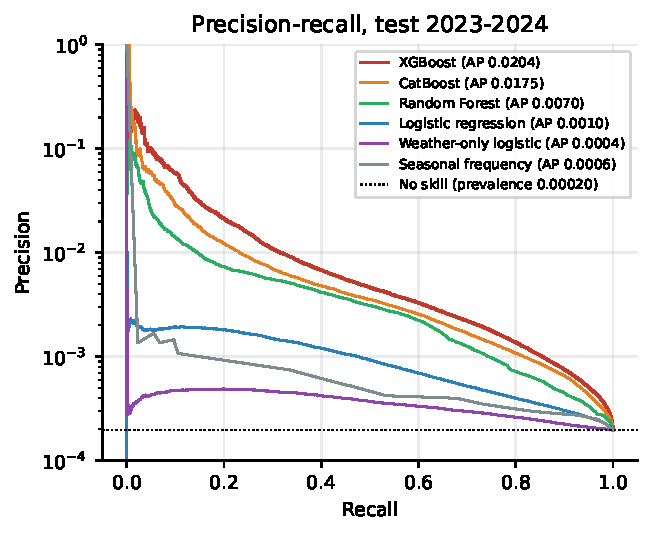
\includegraphics[width=0.85\textwidth]{figures/F1_precision_recall.pdf}
\caption{Precision--recall curves on the test years 2023--2024; the dotted line marks the no-skill precision (prevalence).}\label{fig:pr}
\end{figure}

The gap between logistic regression (AP 0.0010) and the tree ensembles shows that the gain depends on nonlinear interactions, for example among population, land cover, and season, rather than on additive effects. This agrees with regional studies in which gradient boosting performed well on tabular multisource data \cite{jadouli2024morocco,ouazri2026catboost}. As \cite{biswas2025geoai} cautions, it does not imply that deeper architectures are required.

\textbf{Answer to RQ1 (performance).} Combining multisource predictors substantially and significantly improves next-day prediction over both the seasonal-frequency and the weather-only references.

\subsection{Added value of predictor groups}\label{sec:res_ablation}

To identify where this improvement originates, XGBoost was refitted with one predictor group removed at a time, using the frozen hyperparameters (Table~\ref{tab:ablation}, Fig.~\ref{fig:ablation}). Removing terrain caused the largest loss, 0.0154 AP (0.0118--0.0233). Land cover (0.0094), human pressure (0.0079), and season (0.0045) followed, and all three losses were significant. Removing vegetation or the 7/14-day weather windows produced no significant change. Removing daily weather slightly increased AP ($-0.0068$; $-0.0144$ to $0.0011$). A model trained on weather alone reached an AP of only 0.0006, close to the weather-only logistic reference. Rolling validation agreed: terrain was again the largest loss (mean AP 0.0096 against 0.0159).

\begin{table}[htbp]
\caption{Predictor-group ablation of XGBoost (frozen hyperparameters, refitted)}\label{tab:ablation}
\centering\footnotesize
\setlength{\tabcolsep}{3pt}
\begin{tabularx}{\textwidth}{@{}l >{\centering\arraybackslash}X >{\centering\arraybackslash}X >{\centering\arraybackslash}X >{\centering\arraybackslash}X@{}}
\toprule
Variant & Inputs & Test AP & AP lost (95\% CI) & Rolling-validation mean AP \\
\midrule
Full model & 26 & 0.0234 & -- & 0.0159 \\
Without daily weather ($t-7$) & 20 & 0.0303 & $-$0.0068 ($-$0.0144, 0.0011) & 0.0166 \\
Without 7/14-day weather & 22 & 0.0241 & $-$0.0007 ($-$0.0082, 0.0029) & 0.0162 \\
Without vegetation & 23 & 0.0211 & 0.0023 ($-$0.0028, 0.0062) & 0.0156 \\
Without land cover & 21 & 0.0140 & 0.0094 (0.0021, 0.0134) & 0.0150 \\
Without terrain & 22 & 0.0081 & 0.0154 (0.0118, 0.0233) & 0.0096 \\
Without human pressure & 24 & 0.0155 & 0.0079 (0.0002, 0.0123) & 0.0145 \\
Without season & 24 & 0.0190 & 0.0045 (0.0006, 0.0076) & 0.0144 \\
Weather only & 10 & 0.0006 & 0.0228 (0.0184, 0.0321) & 0.0018 \\
\bottomrule
\end{tabularx}
\par\smallskip\raggedright\scriptsize Post hoc analysis after the final test; it explains the result and selects nothing.
\end{table}
\begin{figure}[htbp]
\centering
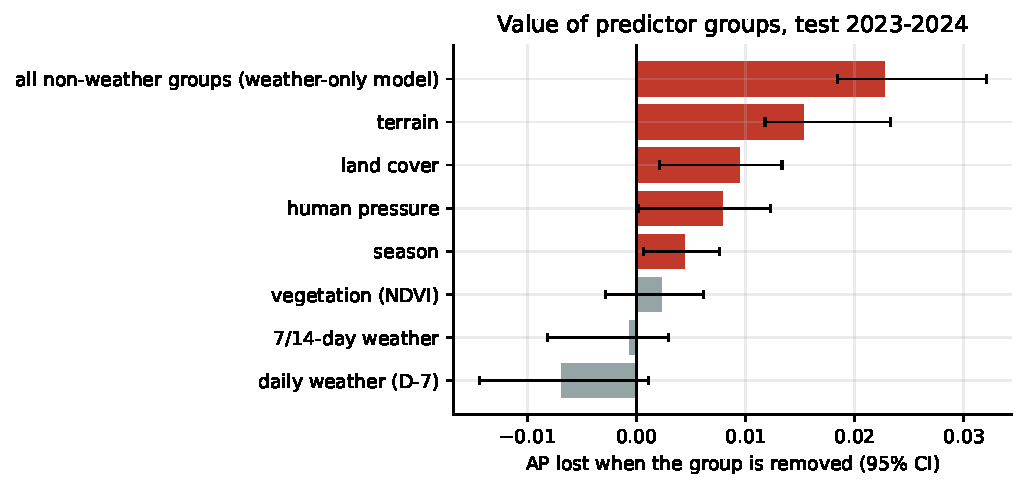
\includegraphics[width=0.85\textwidth]{figures/F14_ablation.pdf}
\caption{Average precision lost when each predictor group is removed (test 2023--2024, paired 95\% intervals); red bars exclude zero.}\label{fig:ablation}
\end{figure}

This outcome was not expected from weather-driven danger systems \cite{kondylatos2022danger}. Two explanations are plausible. First, the seven-day weather lag removes the short-term variability that controls fuel drying, so the compound drought--heat conditions described for Central Asia \cite{ding2026vegetation} cannot be resolved in time. Second, ignitions in the Kazakh steppe are dominated by human activity, such as agricultural and pasture burning, whose location and timing are captured by land use, population, and the calendar \cite{jones2022fireclimate,iban2024shap}.

\textbf{Answer to RQ1 (predictor groups).} The improvement comes mainly from terrain, land-cover, human, and seasonal information. As implemented, the lagged weather and vegetation predictors added no measurable value.

\subsection{Temporal and geographic transfer}\label{sec:res_transfer}

Temporal transfer was stable (Table~\ref{tab:transfer}). AP was 0.0192 in 2023 and 0.0277 in 2024, ROC-AUC was 0.92 in both years, and validation AP had been 0.0191. Geographic transfer was markedly weaker. In the five spatial-block folds, mean AP fell to 0.0039, which is 15 times the no-skill level (range 6--37), compared with 104 times on the temporal test. Ranking ability remained (ROC-AUC 0.81--0.89), but Brier skill was negative in four of five folds.

\begin{table}[htbp]
\caption{Temporal and geographic transfer of XGBoost}\label{tab:transfer}
\centering\footnotesize
\setlength{\tabcolsep}{3pt}
\begin{tabularx}{\textwidth}{@{}l >{\centering\arraybackslash}X >{\centering\arraybackslash}X >{\centering\arraybackslash}X >{\centering\arraybackslash}X@{}}
\toprule
Evaluation & AP & AP/prevalence & ROC-AUC & BSS \\
\midrule
Rolling validation 2019--2021 (mean) & 0.0191 & -- & -- & -- \\
Temporal test 2023 & 0.0192 & 80 & 0.924 & $-$0.006 \\
Temporal test 2024 & 0.0277 & 181 & 0.923 & 0.010 \\
Temporal test 2023--2024 & 0.0204 & 104 & 0.924 & 0.000 \\
Spatial fold 1 & 0.0005 & 6 & 0.808 & $-$0.048 \\
Spatial fold 2 & 0.0083 & 37 & 0.882 & 0.001 \\
Spatial fold 3 & 0.0043 & 12 & 0.890 & $-$0.022 \\
Spatial fold 4 & 0.0030 & 10 & 0.859 & $-$0.004 \\
Spatial fold 5 & 0.0031 & 12 & 0.890 & $-$0.010 \\
Spatial folds (mean) & 0.0039 & 15 & 0.866 & $-$0.017 \\
\bottomrule
\end{tabularx}
\par\smallskip\raggedright\scriptsize Spatial folds: 100\,km blocks with a 25\,km buffer, development period, hyperparameters fixed.
\end{table}

Reviews identify distribution shift across regions as a persistent obstacle \cite{xu2025deep,ejaz2025pipeline,galvanlara2026systematic}. The ablation suggests a mechanism. The strongest predictors locate habitually burning places, and this knowledge is local, so it transfers poorly to regions the model has not seen. Because hyperparameters were fixed globally, the spatial audit is conditional rather than fully nested.

\textbf{Answer to RQ2.} The models generalize well to future years. In geographically separate regions they retain a useful ranking but lose most of their precision and probability skill, which indicates a need for regional calibration or retraining.

\subsection{Calibration and spatial prioritization}\label{sec:res_calibration}

After sigmoid calibration on 2022, the expected calibration error was very small (about $8\times10^{-5}$), but only because nearly all probabilities are close to zero. Brier skill relative to the seasonal reference was close to zero for every model (XGBoost 0.0002; CatBoost 0.0085). The four map classes ordered risk correctly: observed frequency rose from $9\times10^{-6}$ to $2.6\times10^{-3}$ (Table~\ref{tab:classes}). However, they over-predicted by a factor of 1.3--1.8. Above a probability of 0.1, each reliability bin held 143 cell-days or fewer, and observed frequencies were erratic (Fig.~\ref{fig:reliability}). At the 2022 threshold of 0.047, XGBoost alerts were correct 9.8\% of the time and covered 5.2\% of starts, so 90\% of alerts were false. Accuracy (0.9997) is uninformative at this prevalence.

\begin{table}[htbp]
\caption{XGBoost map classes fixed on 2022: predicted and observed frequency, 2023--2024}\label{tab:classes}
\centering\footnotesize
\setlength{\tabcolsep}{3pt}
\begin{tabularx}{\textwidth}{@{}l >{\centering\arraybackslash}X >{\centering\arraybackslash}X >{\centering\arraybackslash}X >{\centering\arraybackslash}X >{\centering\arraybackslash}X@{}}
\toprule
Class & Probability range & Cell-days ($\times10^{6}$) & Mean predicted & Observed & Predicted/observed \\
\midrule
1 & 0 -- $4.8\times10^{-5}$ & 39.8 & $1.2\times10^{-5}$ & $9.0\times10^{-6}$ & 1.33 \\
2 & $4.8\times10^{-5}$ -- $2.3\times10^{-4}$ & 25.3 & $1.2\times10^{-4}$ & $6.7\times10^{-5}$ & 1.82 \\
3 & $2.3\times10^{-4}$ -- $7.9\times10^{-4}$ & 11.0 & $3.9\times10^{-4}$ & $3.0\times10^{-4}$ & 1.28 \\
4 & $7.9\times10^{-4}$ -- 1 & 4.0 & $3.4\times10^{-3}$ & $2.6\times10^{-3}$ & 1.32 \\
\bottomrule
\end{tabularx}
\end{table}
\begin{figure}[htbp]
\centering
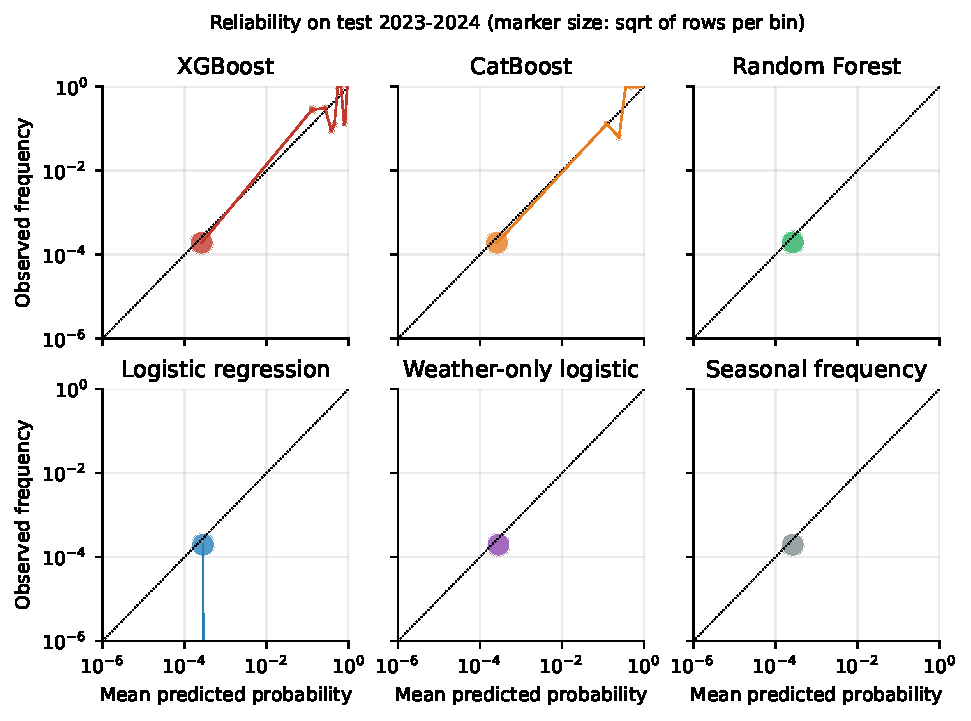
\includegraphics[width=0.85\textwidth]{figures/F3_reliability.pdf}
\caption{Reliability diagrams on the test years; marker size grows with the number of cell-days per bin.}\label{fig:reliability}
\end{figure}

The systematic over-prediction is consistent with the declining prevalence. The calibration year had a prevalence of $2.5\times10^{-4}$, against $2.4\times10^{-4}$ in 2023 and $1.5\times10^{-4}$ in 2024. The pattern also mirrors the warning of \cite{choi2026burnedarea} that a small aggregate calibration error can conceal unreliable high-probability bins. The classes therefore support the class-based mapping proposed by \cite{apostolakis2025interpretation} as relative priority levels, not as absolute chances.

\textbf{Answer to RQ3 (calibration).} The probabilities are reliable as a ranking and on average, but not in magnitude. They need recalibration, preferably seasonal and regional, before they can be used as absolute probabilities.

\subsection{Model explanations across land cover and regions}\label{sec:res_shap}

The largest global TreeSHAP contributions came from population density (0.59), the cosine of the month (0.41), 14-day temperature (0.40), cropland fraction (0.33), and elevation (0.30) (Fig.~\ref{fig:shap}). The driving groups differed by land cover (Table~\ref{tab:landcover}). Cropland outputs depended most on antecedent weather and land cover, which is consistent with weather-timed stubble burning. Grassland outputs depended on human pressure and season, and forest outputs on land cover, antecedent weather, and human pressure. Grassland held 81\% of the test starts and reached an AP of 0.041. Cropland reached only 0.013, and forest-dominated cells recorded just five starts. Regionally, AP ranged from 0.163 in Atyrau and 0.121 in Aktobe down to 0.0006 in Akmola and 0.0024 in Kostanay, where widespread cropland burning is hard to anticipate cell by cell.

SHAP ranks 14-day temperature highly even though the ablation shows that antecedent weather is replaceable. Temperature is strongly correlated with season, and SHAP distributes credit among correlated predictors. This confirms that explanations describe predictive associations rather than causes \cite{iban2024shap,ouazri2026catboost}. Population density as the leading predictor agrees with the human-access drivers emphasized in previous studies \cite{iban2024shap,bouzeraa2025wsm}.

\textbf{Answer to RQ3 (explanations).} The outputs are explained mainly by human, seasonal, and land-surface factors, and the dominant factors change between land-cover groups and regions.

\begin{table}[htbp]
\caption{XGBoost performance and leading SHAP groups by dominant land cover, 2023--2024}\label{tab:landcover}
\centering\footnotesize
\setlength{\tabcolsep}{3pt}
\begin{tabularx}{\textwidth}{@{}l >{\centering\arraybackslash}X >{\centering\arraybackslash}X >{\centering\arraybackslash}X >{\centering\arraybackslash}X X@{}}
\toprule
Land cover & Test starts & AP & AP/prev. & BSS & Leading predictor groups (mean $|$SHAP$|$) \\
\midrule
Grassland & 12,805 & 0.0413 & 225 & 0.016 & human 0.65; season 0.61; antecedent weather 0.57 \\
Cropland & 1,947 & 0.0134 & 21 & 0.005 & antecedent weather 1.15; land cover 0.81; season 0.44 \\
Other & 947 & 0.0359 & 263 & $-$0.228 & land cover 1.20; terrain 0.77; human 0.73 \\
Forest & 5 & 0.0014 & 40 & $-$0.005 & land cover 0.94; antecedent weather 0.81; human 0.73 \\
Shrubland & 0 & -- & -- & -- & land cover 1.75; weather 0.74; season 0.47 \\
\bottomrule
\end{tabularx}
\par\smallskip\raggedright\scriptsize SHAP values are in uncalibrated log-odds and describe predictive associations, not causes.
\end{table}
\begin{figure}[htbp]
\centering
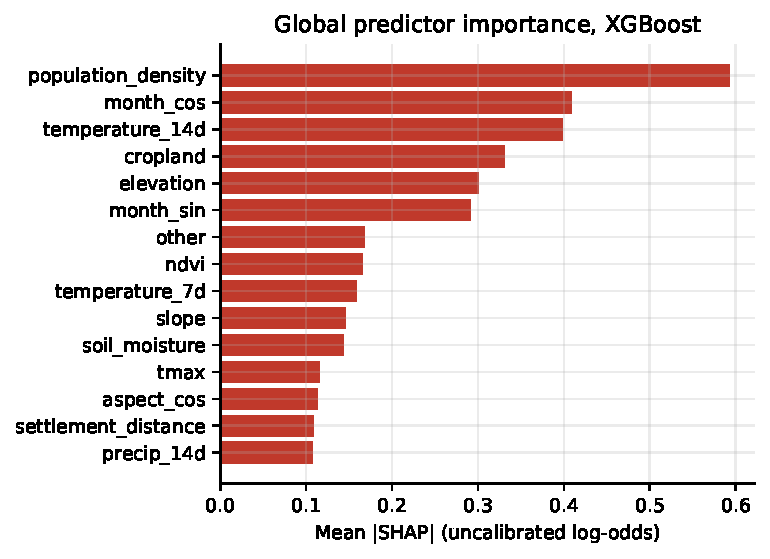
\includegraphics[width=0.85\textwidth]{figures/F5_shap_global.pdf}
\caption{Global TreeSHAP importance of the fifteen strongest predictors of XGBoost.}\label{fig:shap}
\end{figure}

\subsection{Case study: the June 2023 Abay Region fire}\label{sec:res_case}

Between 7 and 9 June 2023, 19--31\% of each day's new starts fell inside that day's top 5\% of cells (Fig.~\ref{fig:case}). The start near Semei on 8 June ranked at the 78th percentile and was therefore not flagged, whereas four of the seven other eastern starts on 8--9 June ranked at or above the 96th percentile. The model would not have singled out the start of the motivating disaster \cite{sentinel2023abayfire}. This supports the caution stated in the Introduction and the distinction between occurrence probability and risk \cite{dossi2026infrastructure,berchtold2025tipping}.

\begin{figure}[htbp]
\centering
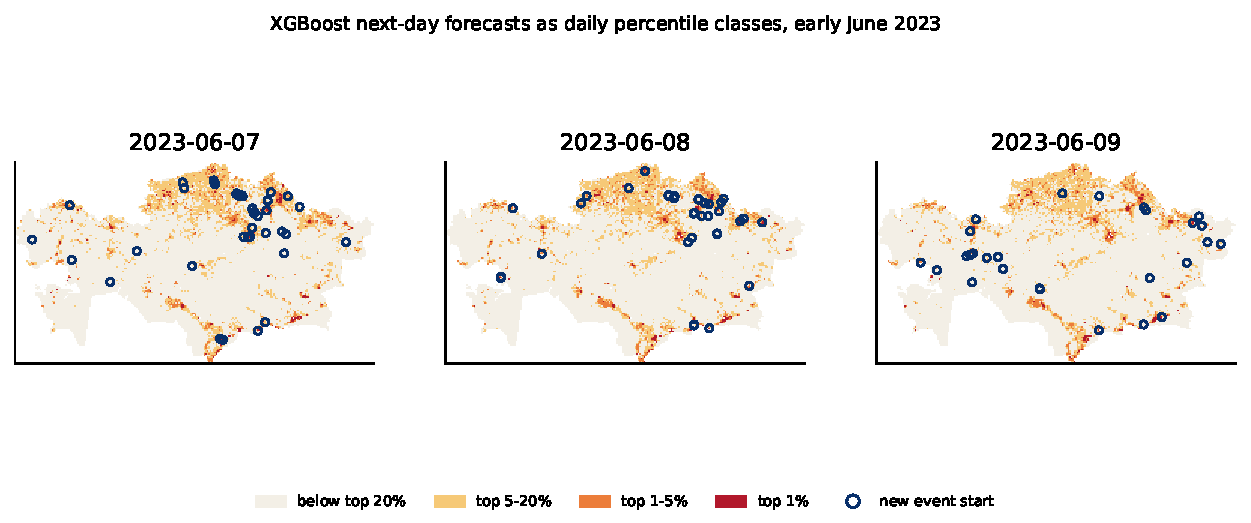
\includegraphics[width=0.85\textwidth]{figures/F13_case_june_2023.pdf}
\caption{Next-day forecasts for 7--9 June 2023 as daily percentile classes, with the new event starts of each day.}\label{fig:case}
\end{figure}

\subsection{Practical implications and limitations}\label{sec:res_limits}

In practice, the framework is most useful as a prioritization tool. Inspecting the top 5\% of cell-days covers more than half of all new starts, and the fixed map classes can serve as relative alert levels. Compared with the national static hazard maps \cite{babu2025sfri,chepashev2025maxent}, the results confirm that static land-surface and human layers carry most of the predictable signal. They also add a daily time dimension, temporal testing, and calibration evidence.

Several limitations remain. The labels come from a single sensor and record active-fire detections rather than ignitions. Agricultural burning cannot be separated from wildfire, and residual persistent heat sources may inflate some western regional scores. Weather enters with a seven-day lag. Tuning used five rather than fifty trials, and the spatial audit was conditional. Forest fires are too rare at 5\,km for reliable evaluation. Three outcomes were unexpected: weather added no value, CatBoost produced the best Brier skill, and 2024 scored higher than 2023 despite its lower prevalence.

\section{Conclusion}\label{sec:conclusion}

This study developed and evaluated an explainable multisource machine-learning framework for next-day prediction of new vegetation-fire starts on a 5\,km grid covering Kazakhstan. Models were trained on 2015--2021, calibrated on 2022, and tested on the untouched years 2023--2024 against seasonal-frequency and weather-only references. XGBoost performed best: its average precision of 0.020 was about one hundred times the no-skill level and significantly higher than both references, and the top 5\% of its daily scores captured more than half of all new fire starts. Skill remained stable from the validation years to the test years.

The results also qualify these gains. Most predictive information came from terrain, land cover, human pressure, and season, whereas weather available with a realistic seven-day delay and vegetation indices added no measurable value. The models transferred well to future years but much less well to unseen regions. The calibrated probabilities ranked locations reliably, but their magnitudes were biased under declining fire prevalence. The SHAP explanations showed that the drivers differ between cropland, grassland, and forest. A retrospective look at the June 2023 Abay fire showed that the model would not have singled out its starting location.

The main contribution of the study lies in reporting all of these results together for Kazakhstan: rare-event metrics with uncertainty intervals, separate temporal and geographic transfer tests, calibration diagnostics, grouped ablations, and explanations stratified by land cover and region. Taken together, they show where a daily forecast is useful, namely as a ranking tool that directs attention to the most likely ignition areas, and where it is not yet reliable, namely as an absolute probability or in regions absent from training. These distinctions matter for emergency services that may use such maps to plan monitoring and prevention.

Future work should add numerical weather forecasts for the target day so that meteorology is no longer seven days old. It should also combine detections from several satellites, separate agricultural burning from uncontrolled wildfires, and recalibrate probabilities by season and region. A finer grid in forest zones would allow forest fires to be evaluated separately. Finally, prospective validation with forecasts issued before each day, corroborated by burned-area products and official incident records, would test whether the reported skill holds in operational use.

\bibliography{references}
\end{document}
